\documentclass{article} % For LaTeX2e
\usepackage{nips15submit_e,times}
\usepackage{hyperref}
\usepackage{url}
\usepackage{graphicx} 
\usepackage{amsmath}
\usepackage{chngpage}
\usepackage{float}
%\documentstyle[nips14submit_09,times,art10]{article} % For LaTeX 2.09


\title{Road Estimation Using Machine Learning Algorithms}


\author{
Zili Chen\\
Department of Computer Science\\
University of Toronto\\
Toronto, ON\\
\texttt{zlchen@cs.toronto.edu} \\
\And
Chenguang Zhu\\
Department of Computer Science\\
University of Toronto\\
Toronto, ON\\
\texttt{zhuchenguang.zhu@mail.utoronto.ca} \\
}


\newcommand{\fix}{\marginpar{FIX}}
\newcommand{\new}{\marginpar{NEW}}

\nipsfinalcopy % Uncomment for camera-ready version

\begin{document}


\maketitle

\begin{abstract}
In real world, road detection is becoming more and more important when implementing autonomous driving system. The goal of this project is to create a classifier  that is able to create a pixel-wise segmentation whether the given image is a road or not (i.e., binary classification). However, labeling each pixel needs huge computation. To solve this problem, we use SLICO (Zero Parameter version of Simple Linear Iterative Clustering), which first computes super-pixels for each image to ease the computation. \\

For the purpose of investigating machine learning techniques to solve this task, we apply pixel-wised approach to tackle this problem and use various machine learning methods to perform experiments, including K-NN, RBF-kernel SVM, AdaBoost, RandomForest, Bagging and Naive Bayes. Furthermore, considering the influence of neighbor super-pixels, Conditional Random Field is used to improve the performance based on previous predictions. The evaluation is conducted on both super-pixel and pixel level. In our experiments, RandomForest, RBF-kernel SVM and Bagging can produce top results. CRF can always improve the accuracy and smooth the results of basic models. 
\end{abstract}

\section{Introduction}
Detecting the road area ahead of a vehicle is essential for modern driver assistance systems and navigation. However, road detection is a difficult task due to various factors, including the absence of road edge markings, variations in lighting conditions, different road surface materials, occlusions with other vehicles and objects, etc.\\

Although pixel-wise descriptors are widely used in object recognition tasks for image description, it has the problem of scaling. When there is a huge number of image inputs, the performance of classifier is limited  due to large computation burden. Furthermore, it has limitations on dealing with road detection task because it can not take advantage of information of textures or edges of roads. 

\subsection{Related Work}
In the past few years, some classification-based detection methods, which take the color, texture and coordination as the features [1], have been proposed to detect a road based on combining boundaries and area information. Sha[2] proposed the feature combination method for the road detection. His/her method firstly constructed an over-completed feature set on several linear and non-linear combined functions. Foedisch [3] developed an adaptive road detection system based on color histograms using neural network. Alon [4] combined the Adaboost-based region segmentation and the boundary detection constrained by geometric projection to find drivable road area. Chern [5] proposed the image segmentation by the region growing technique. For each region, there are four kinds of features: the coordinate, the color, the luminance and the size. This method can efficiently detect roads but is only applied in well-structured road or highways.

\subsection{Motivations and Objectives}
The goal of this project is to investigate machine learning techniques that are more appropriate to create a pixel wise segmentation of the image in terms of what is road and what is non-road. To ease the computation, we use Zero Parameter version of Simple Linear Iterative Clustering (SLICO) [9] to preprocess the input images to generate super-pixels. \\

The classification task is based on super-pixels, considering each super-pixel as a data example. We use RGB values, locations and the size of the super-pixel as features. \\

We run experiments on the preprocessed data and compare different kinds of classification models, such as K-Nearest Neighbors (K-NN), RBF-Support Vector Machine (RBF-SVM), Gaussian Naive Bayes, ensemble methods, etc. In addition, with regard to correlation between super-pixels, we also use structured prediction method -- Conditional Random Field.

\section{Machine Learning Techniques}
\label{gen_inst}

\subsection{K-Nearest Neighbors}
K-Nearest Neighbors algorithm (K-NN) is a non-parametric classification method that considers the k closest training examples in the feature space as input and class membership as output.\\

In our experiments, the classification decision is made based on the major class membership of the k nearest samples. We eventually choose k=15 as the best parameter of K-NN classifier. 

\subsection{RBF-kernel SVM}
Support vector machines (SVM) are supervised learning models with associated learning algorithms that is extensively used for classification analysis. SVM can efficiently perform a non-linear classification using kernel function. We use RBF kernel in our experiments, which can be written as
\begin{equation}
K(x, x') = exp(-\frac{\left \| x-x' \right \|^{2}}{2\sigma ^{2}})
\end{equation}
In eqution 1, ${\left \| x-x' \right \|^{2}}$may be recognized as the squared Euclidean distance\, between the two feature vectors. ${\sigma}$ is a free parameter. An equivalent but simpler, definition involves a parameter $\gamma = \frac{1}{2\sigma ^{2}}$.\\
This kernel function maps the non-linear separable inputs into high-dimensional feature spaces. It contributes to improving the classification capability of SVM.

\subsection{Ensemble Methods}
Ensemble of classifiers is a set of classifiers whose individual decisions combined in some ways to classify all examples together. In our experiments, we use AdaBoost, RandomForest and Bagging.\\

AdaBoost can be used in conjunction with many other types of learning algorithms to improve their performance [6]. The output of weak classifiers is combined into a weighted sum that represents the final output of the boosted classifier. \\
\begin{equation}
Y^{M}(x)=sign(\sum_{m=1}^{M}\alpha _{m}y_{m}(x)))
\end{equation}
where $\alpha _{m}$ is determined by the error rate of classifier m. \\

RandomForest constructs a multitude of decision trees at training time, and output the class that is the mode of the classes of the individual trees in classification tasks [7]. Random decision forests correct for decision trees’ habit of overfitting to their training set.

\subsection{Gaussian Naive Bayes}
Naive Bayes classifiers are generative classifiers based on applying Bayes' theorem with conditional independence assumptions between the features.\\

The decision function of Naive Bayes classifier is to find the class k that maximizes the joint probability of $x$ and $C _{k}$.\\
\begin{equation}
y=\underset{k}{argmax\,p(t=k))}\prod_{i=1}^{d}p(x_i|t=k)
\end{equation}
In our experiment, we choose Gaussian Naive Bayes, in which the class likelihood follows Gaussian distribution, as one of our classifiers.

\subsection{Conditional Random Field}
Conditional random fields (CRFs) are a class of statistical modelling method often applied in pattern recognition and machine learning,where they are used for structured prediction [8]. Whereas an ordinary classifier predicts a label for a single sample without regard to "neighboring" samples, a CRF can take context into account.\\

In Graph ${G=(V,E)}$, ${Y=(Y_v), v\in V}$--$Y$ is indexed by the vertices of $G$. Then ${(X,Y)}$ is a conditional random field when the random variables $Y_v$, conditioned on $X$, obeying the Markov property with respect to the graph G: \\
\begin{equation}
p(Y_v|X,Y_v,w\neq v)=p(Y_v|X,Y_v,w\sim v)
\end{equation}

where $w\sim v$ means w and v are neighbors in G. What this means is that a CRF is an undirected graphical model whose nodes can be divided into exactly two disjoint sets $X$ and $Y$, the observed and output variables, respectively; the conditional distribution ${p(Y|X)}$ is then modeled.\\

CRF can be added into our models based on previous classifiers outputs to improve performance, by considering the correlations between neighbors (pairwise). In this way, it can reduce the sensitivity to noises through extra new information.

\section{Experiment and Evaluation}
\label{headings}

\subsection{Experiment}
\subsubsection{Dataset and Data preprocessing}
We use the KITTI [11] dataset for experiments. The full dataset includes labeled training data and unlabeled test data, we only use training data to run our tests.There are 289 images in training data. We separate them into three datasets: train (60\%), validation (10\%), test (30\%).\\

We need to ease the computation because the number of pixels per image could be huge (Since the resolution of images are about 375 X 1240. So there are more than 465,000 pixels per image), which lead to lengthy computation time if we apply complex methods to the data. Therefore, we firstly compute super-pixels using SLICO for each image. \\

After SLICO preprocessing, the average labels of super-pixels become float numbers in the range of [0, 1]. We define a threshold of 0.5 to decide the labels of super-pixels because this is a binary classification problem. If the prediction output is larger than 0.5, then it is determined as 1, which means it is road. Otherwise it is determined as 0, which means it is not road. 

\subsubsection{Implementation}
We use scikit-learn [11], a machine learning library in python for implementing our classification models and performing experiments. \\
Scikit-learn provides a large number of machine learning models including all the models we choose in our experiments. They are:
\begin{adjustwidth}{2em}{0em}
$ \bullet  $	K-NN\\
$ \bullet  $	RBF-Kernel SVM\\
$ \bullet  $	AdaBoost\\
$ \bullet  $	RandomForest\\
$ \bullet  $ 	Bagging\\
$ \bullet  $ 	Gaussian Naive Bayes\\
\end{adjustwidth}
Each function has a list of parameters to construct the models so as to fit the input data. We use another library Pystruct [12] to perform our Conditional Random Field learning algorithms. 

\subsection{Evaluation}
\subsubsection{Evaluation Metrics}
We evaluate the results both on super-pixel level and on pixel level for most of experiments. To compare the performance of different approaches, we use Score (Accuracy) as the major metrics.\\
\begin{equation}
Accuracy=\frac{TP+TN}{TP+TN+FP+FN}
\end{equation}
Where TP stands for True Positive, TN stands for True Negative, FP stands for False Positive and FN stands for False Negative.\\

We also use some other commonly-used metrics for evaluating performance, including Precision, Recall and F1 Score.\\
\begin{equation}
Precision = \frac{TP}{TP+FP}
\end{equation}
\begin{equation}
Recall = \frac{TP}{TP+FN}
\end{equation}
\begin{equation}
F1\,Score = 2\frac{Precision*Recall}{Precision+Recall}
\end{equation}

\subsubsection{Segment Selection}
Since the road should always be continuous and has no isolated super pixels, using super-pixels for preprocessing to ease the computation will not affect the classification result too much. However, losses must be taken into consideration because of imperfect super-pixel segmentation.\\

In SLICO preprocessing step, the major parameter for deciding the final outcome of segmentation is the number of super-pixels in each picture. After experimenting with a couple of different number of segments, we obtain Table 1, which compares the classification performance and computation time of models (we use K-NN, K=15 as the example) based on different number of segments.\\
\begin{table}[h]
\centering
\caption{Comparison on Different Number of Segments}
\begin{tabular}{lclclclc|}
\\
\textbf{Segment} &\textbf{Score (Super Pixel)} &\textbf{Score (Pixel)} &\textbf{Time} \\
\\ \hline \\
200	 &93.14\%	 &92.98\%	 &3.251228 \\
400	 &93.73\%	 &92.86\%	 &5.036737 \\
1000	 &94.37\%	 &93.58\%	 &13.175207 \\
2000	 &94.42\%	 &93.67\%	 &41.202781 \\
\end{tabular}
\end{table}
\\
From Table 1, we can tell that when segment = 1000, we get the most appropriate result. When the number of segment is small, for example, 200 and 400, the score is low. When the number of segments is increased from 400 to 1000, we find that the score get 0.64\% promoted. However, if we keep increasing the number of segments, the computation time would grow considerably (from 13.17sec to 41.20sec), but the score only get improved slightly (0.05\% from 1000 to 2000). Overall, taking both accuracy and time into account, 1000 is the best number of segments that we ever get.So we choose number of super-pixels = 1000 as the parameters of our SLICO segmentation process.\\ 

\subsubsection{Feature Selection}
The selection of features need to be done before using classifiers to deal with road detection task. Actually, feature extraction can be considered as a step of data preprocessing. Since super-pixels are formed by aggregating single pixels, the most straightforward way seems to be taking the average RGB values of a super-pixel as its features. However, in fact, pixels have more information than just RGB values. For example, the location of a pixel can be very important when determining whether the pixel is road or not. Therefore, we add location information, which are average x, and y coordinates, into features. \\

Furthermore, the size of each super-pixel could also provide useful information because each super-pixel consists of a number of single pixels. Therefore, we add super-pixel size into features.\\
\begin{table}[h]
\centering
\caption{Comparison on Different Number of Features}
\begin{tabular}{lclclclc|c|c|c|}
\\
&\multicolumn{2}{|c|}{\bf 3 Features} & \multicolumn{2}{|c|}{\bf 5 Features} & \multicolumn{2}{|c|}{\bf 6 Features} \\
\\ \hline \\
&\textbf{SuperPixel} &\textbf{Pixel} &\textbf{SuperPixel} &\textbf{Pixel} &\textbf{SuperPixel} &\textbf{Pixel} \\
\\
K-NN	 		 &90.27\% &89.90\% &93.97\% &93.21\% &94.37\% &93.58\% \\
GaussianNB	 &84.59\%	 &84.80\%	 &89.71\% &89.44\% &89.82\% &89.54\% \\
Bagging 		 &89.90\%	 &89.57\%	 &94.67\% &93.86\% &94.67\% &93.87\% \\
AdaBoost 		 &83.63\%	 &83.82\%	 &93.72\% &93.05\% &93.89\% &93.16\% \\
RandomForest  &90.11\%	 &89.77\%	 &94.87\% &94.00\% &94.91\% &94.05\% \\
RBF-SVM		 &89.98\%	 &89.60\%	 &94.78\% &93.98\% &94.90\% &94.08\% \\
\end{tabular}
\end{table}
\\
Now we have 6 features (R, G, B, x, y, and size), which form a feature set for each super-pixel. From the result of our experiments in Table 2, we can easily draw a conclusion that 6 features yield the best prediction under most classifiers.\\

On validation set, from Figure 1, we can find that among all the models we experimented, Bagging, RandomForest and RBF-kernel SVM have top performance because they produce highest scores. Gaussian Naive Bayes has the worst performance. All classifiers perform better with 6 features than with 5 features or 3 features.\\
\begin{figure}[htbp]
\centering
\begin{minipage}{2.65in}
\centering
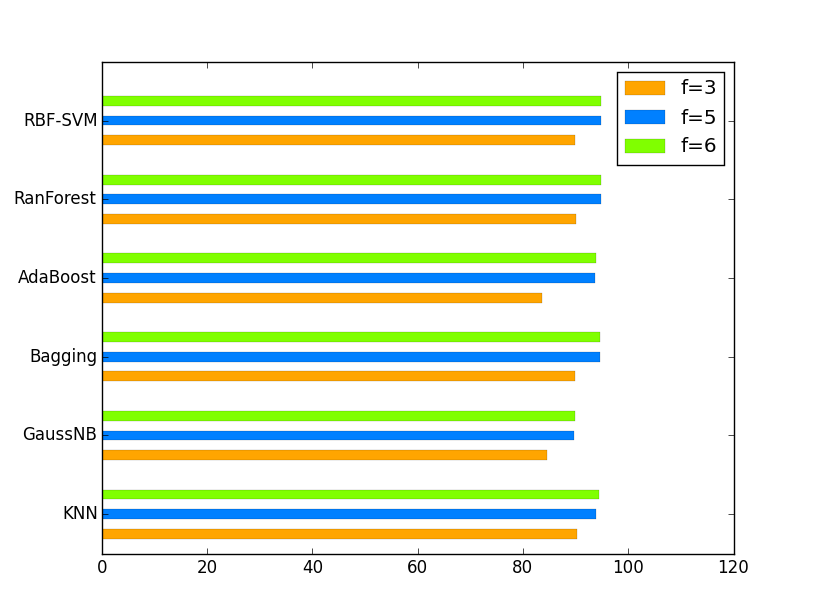
\includegraphics[width=1.1\textwidth]{1.png}
\caption{Different Features  (Super-Pixel)}
\end{minipage}
\begin{minipage}{2.65in}
\centering
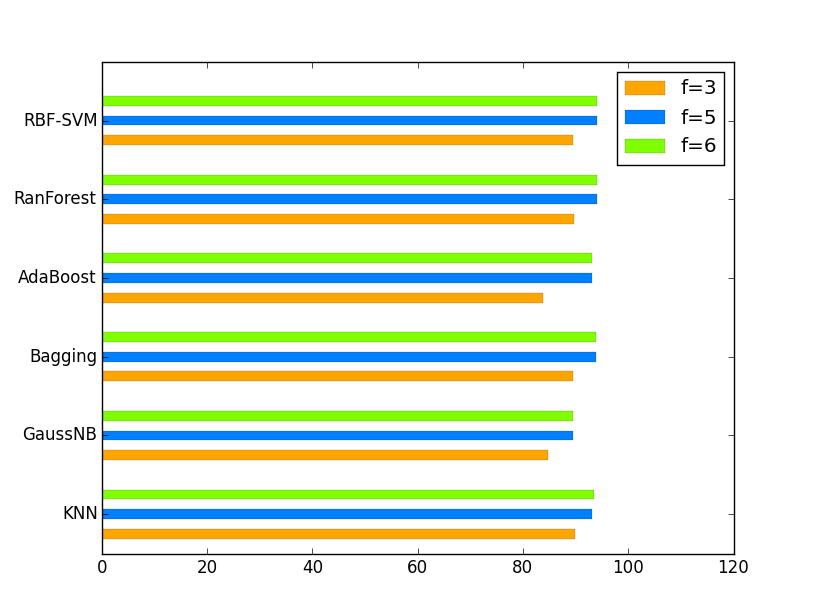
\includegraphics[width=1.1\textwidth]{2.png}
\caption{Different Features (Pixel)}
\end{minipage}
\end{figure}
\\
\\
Adding the 7th feature--histogram of oriented gradient seems to have negligible positive influence. And it takes much longer time for computation than using 6 features. Considering the time cost, 6 is the most appropriate number of features for road detection task because when using more than 6 features, although some classifiers yield higher accuracy, the improvement is quite slight. And for most of the classifiers, 7 features does not have positive influence on their scores. Furthermore, increasing the number of features to 7 can increase the computation time obviously. Therefore, 6 features turn out to be the best feature set when taking both scores and speed into consideration. In the following evaluations, we all use 6 features as the feature set.

\subsubsection{Parameter Selection}
After deciding features, we test performance on different datasets by adjusting the parameters of each classifier and observe the variation of accuracy.\\

We use K-NN, RBF-kernel SVM and RandomForest as example models to perform the following experiments.\\

For each model, these are parameters we adjust: K for K-NN, error penalty term C for RBF-kernel SVM, and number of individual classifiers n for RandomForest.\\
\begin{figure}[h]
\centering
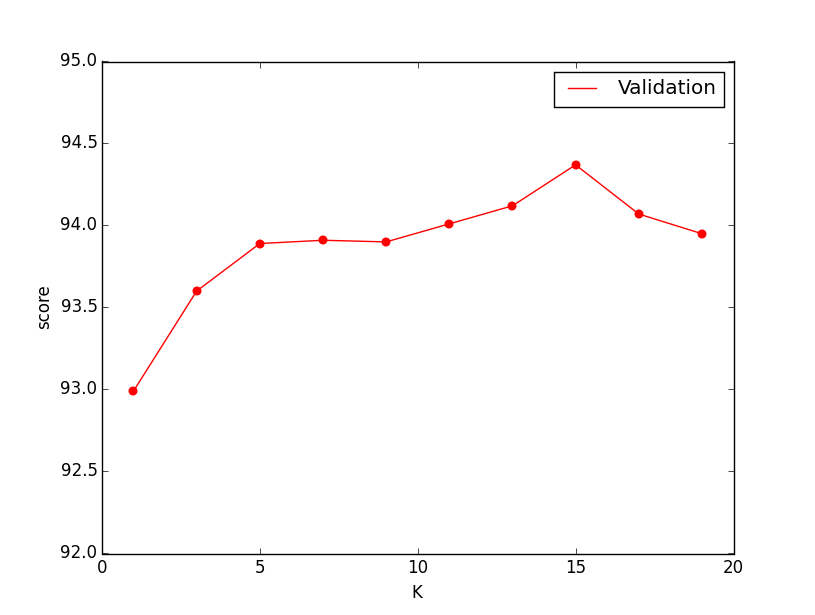
\includegraphics[width=0.5\textwidth]{3.png}
\caption{Performance of K-NN}
\end{figure}

For K-NN, as K becomes larger, the accuracy on validation set firstly grows up then starts descending after K is larger than 15. The accuracy on validation set reaches its peak when K=15. Therefore, 15 is the most appropriate value of K.\\
\begin{figure}[htbp]
\centering
\begin{minipage}{2.65in}
\centering
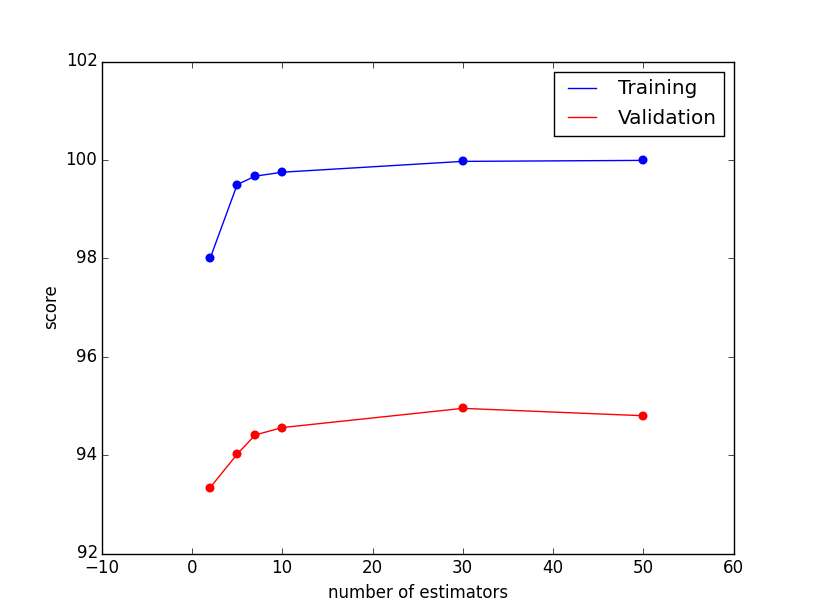
\includegraphics[width=1.1\textwidth]{4.png}
\caption{Performance of RandomForest}
\end{minipage}
\begin{minipage}{2.65in}
\centering
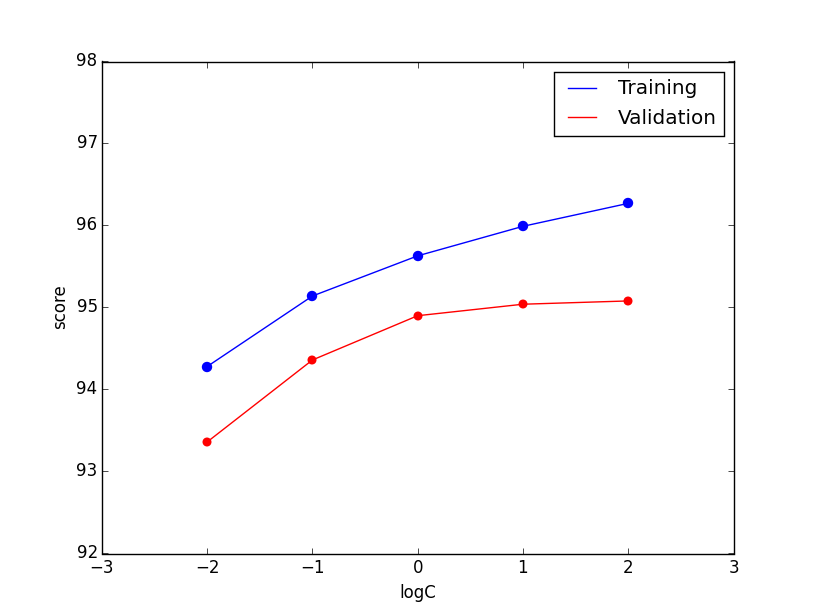
\includegraphics[width=1.1\textwidth]{5.png}
\caption{Performance of RBF-SVM}
\end{minipage}
\end{figure}
\\
For RBF-kernel SVM, we adjust the penalty term C. In Figure 5, we observe that larger C tends to give better results. It means that there are not many noises in the data. When C grows, it can prevent the model from overfitting. Therefore, the performance of RBF-SVM fit is better when C=100.\\

We take RandomForest as the example of ensemble methods, on training set, RandomForest achieves nearly 100\% accuracy after the number of estimators is larger than 30. But on validation set the score decreases when the number of estimators reaches 50, which means overfitting happens due to excessive complexity of model. From our experiments, we find that 30 is the best number of estimators for RandomForest.\\
\begin{table}[h]
\centering
\caption{Score of Three Classifiers on Super-pixel Level and Pixel Level}
\begin{tabular}{lclclclc|}
\\
&\textbf{K-NN} &\textbf{RandomForest} &\textbf{RBF-SVM} \\
\\ \hline \\
Super-Pixel Level	 &94.37\%	 &\quad\; 95.01\%	 &95.08\% \\
Pixel Level	 &93.58\%	 &\quad\; 94.15\%	 &94.25\% \\
\end{tabular}
\end{table}
\\
Using the best parameters selected in previous step for each model, we obtain the score of the 3 classifiers on both super-pixel level and pixel level, as showed in Table 3.

\subsubsection{Conditional Random Field}
Since roads should always be continuous, it is reasonable to take the influence of a pixel's neighbors' labels into consideration when determining its own label. If its neighbors are already classified as road, then this pixel has a very high probability to be road as well. \\

In all of the models we have experimented so far, we cannot take this information into account because they all treat each super-pixel independently. Thus, we use Pairwise CRF on a general graph. Pairwise potentials the same for all edges, are symmetric by default, which leads to n classes parameters for unary potentials. We implement GraphCRF on three different classifiers: Gaussian Naive Bayes, RandomForest and K-NN.\\

We choose these models based on their performance. From our experiments, RandomForest yields best results while Gaussian Naive Bayes has the lowest accuracy. Another classifier we selected is K-NN due to its highest computation speed. The evaluation on both super-pixel-level and pixel-level for the three different models before and after CRF is showed in Table 4. \\
\begin{table}[h]
\centering
\caption{Comparison on Different Number of Features}
\begin{tabular}{lclclclc|c|c|c|}
\\
&\multicolumn{2}{|c|}{\bf K-NN} & \multicolumn{2}{|c|}{\bf GaussianNB} & \multicolumn{2}{|c|}{\bf RandomForest} \\
\\ \hline \\
&\textbf{Before} &\textbf{After} &\textbf{Before} &\textbf{After} &\textbf{Before} &\textbf{After} \\
\\
Valid Score(Super-Pixel)	 &93.97\% &94.79\% &89.82\% &91.06\% &94.80\% &95.68\% \\
Test Score(Super-Pixel)	 &94.37\%	 &95.05\%	 &89.93\% &91.53\% &94.42\% &94.93\% \\
Valid Score(Pixel)	 &93.21\% &N/A &89.54\% &N/A &93.94\% &N/A \\
Test Score(Pixel)	 &93.58\%	 &N/A &89.73\% &N/A &93.88\% &N/A \\
Precision 		 &83.48\%	 &86.01\%	 &71.12\% &71.19\% &91.42\% &90.8\% \\
Recall 		 &88.82\%	 &88.79\%	 &76.29\% &79.51\% &93.82\% &93.47\% \\
F1 Score  	         &86.07\%	 &87.38\%	 &73.62\% &75.12\% &92.61\% &92.12\% \\
\end{tabular}
\end{table}
\\
To use pairwise CRF on a general graph, we have to build pairwise potentials based on the outputs of previous classifiers. If there is one super-pixel corresponds to another one, then we assume there is an undirected edge between them. Besides, pairwise potentials the same for all edges, are symmetric by default, which leads to n classes parameters for unary potentials. Since our experiment is a binary classification problem, we only have n = 2, which means the unary potentials should be a two-dimension feature ${x_1, x_2}$ where ${x_1 + x_2 = 1}$. Currently PyStruct implements only max-margin methods and a perceptron, so we choose structural support vector machines to speed up the convergence.\\
\begin{figure}[htbp]
\centering
\begin{minipage}{2.65in}
\centering

\includegraphics[width=0.9\textwidth]{6.png}
\caption{K-NN before CRF}
\end{minipage}
\begin{minipage}{2.65in}
\centering

\includegraphics[width=0.9\textwidth]{7.png}
\caption{K-NN after CRF}
\end{minipage}
\end{figure}
\begin{figure}[htbp]
\centering
\begin{minipage}{2.65in}
\centering

\includegraphics[width=0.9\textwidth]{8.png}
\caption{Ground Truth}
\end{minipage}
\begin{minipage}{2.65in}
\centering
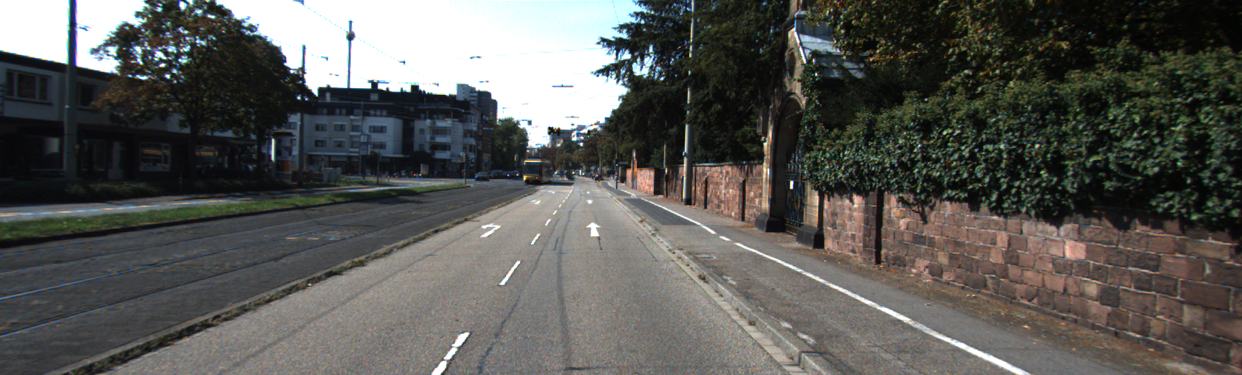
\includegraphics[width=0.9\textwidth]{9.png}
\caption{Original Image}
\end{minipage}
\end{figure}
\\
We select one sample from the dataset to illustrate the performance of our CRF method. Figure 6 is the prediction of K-NN before using CRF while Figure 7 is the prediction result after applying CRF. By comparing their accuracy and their difference from ground truth (Figure 8) and original image (Figure 9), CRF can make more smooth boundaries and produce better prediction performance, which can also be observed by comparing the statistics in Table 4.\\
\begin{figure}[htbp]
\centering
\begin{minipage}{2.65in}
\centering
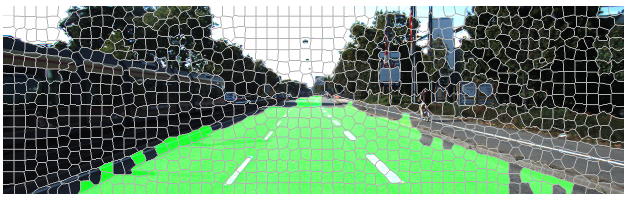
\includegraphics[width=0.9\textwidth]{10.png}
\caption{Prediction before CRF}
\end{minipage}
\begin{minipage}{2.65in}
\centering
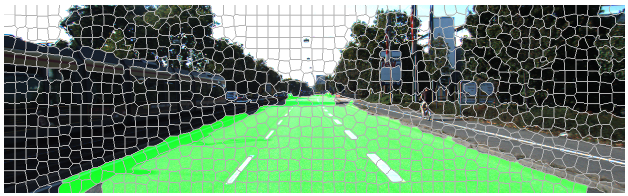
\includegraphics[width=0.9\textwidth]{11.png}
\caption{Prediction after CRF}
\end{minipage}
\end{figure}
\\
In Figure 10 and Figure 11, we combine the prediction of our methods with SLICO-preprocessed images to illustrate the performance of CRF. Green super-pixels are classified as road while others are classified as non-road. It is obvious that after applying CRF we yield better prediction result with smoother boundary and higher accuracy.

\section{Conclusion}
In our experiment, we initially preprocess data by aggregating pixels to generate super-pixels, then determine which features to use, perform experiments using different classification models and use Conditional Random Field to improve the results. 

Among all of our experiments, we achieve a score of over 95\% on super-pixel level, while on pixel level the accuracy is 94\%. To compare the performance of different machine learning models, we experiment a number of classifiers including K-NN, RBF-kernel SVM, AdaBoost, RandomForest, Bagging and Gaussian Naive Bayes. We compare their accuracy and computation time and summary the result.

To improve the performance, we run Conditional Random Field on top of our pervious result. We find that CRF makes the prediction smoother and produce better estimation of road.

There are some improvements can be done in future work, for example, how to reduce the computation time when the number of features increases. We consider that one way to solve this problem is data compression. It can efficiently reduce space and time required, while not losing too much accuracy. Apart from reducing the computation cost, there are some other possible aspects can be explored, such as experimenting some other models (for example, neural networks) and trying more structured prediction techniques.

\newpage

\subsubsection*{References}

\small{
[1] C. Xu, C. Mi, C. Chen, \& Z.B Yang, {\it Road detection based on vanishing point location}, JCIT, vol. 7, no. 6, pp.137-145, 2012

[2] Y. Sha, G.Y Zhang, \& Y. Yang, {\it A road detection algorithm by boosting using feature combination},
In: Proceeding of the 2007 IEEE Intelligent Vehicles Symposium Istanbul, Turkey, June 13-15, 2007

[3] M. Foedisch, \& A. Takeuchi, {\it Adaptive road detection through continuous environment learning},
information theory, In: Proceedings of the International Symposium on ISIT, pp.16-21, 13-15 Oct. 2004

[4] Y. Alon, A. Ferencz, \& A. Shashua, {\it Off-road path following using region classification and geometric projection constraints}, In Proceeding of the IEEE Conference Computer Vision Pattern Recognition, pp. 689-696, 2006

[5] M.Y Chern, \& S.-C Cheng, {\it Finding road boundaries from the unstructured rural road scene}, In: Proceeding of the 16th IPPR Conference on Computer Vision, Graphics and Image Processing (CVGIP) , 2003

[6] Freund, Y. \& Schapire, R. (1997). {\it A Decision-Theoretic Generalization of On-Line Learning and an Application to Boosting}. Journal of Computer and System Sciences, 55(1), pp.119-139.

[7] Ho, Tin Kam (1995). {\it Random Decision Forests (PDF). Proceedings of the 3rd International Conference on Document Analysis and Recognition}, Montreal, QC, 14–16 August 1995. pp. 278–282

[8] Lafferty, J., McCallum, A.,\& Pereira, F. (2001). {\it Conditional random fields: Probabilistic models for segmenting and labeling sequence data}. Proc. 18th International Conf. on Machine Learning. Morgan Kaufmann. pp. 282–289.

[9] R. Achanta, A. Shaji, K. Smith, A. Lucchi, P. Fua, \& S. Susstrunk, {\it Slic superpixels compared to state-of-the-art superpixel methods}, IEEE Trans. Pattern Anal. Mach. Intell., vol. 34, no. 11, pp. 2274-2282, 2012.

[10] R. Urtasun, P. Lenz, \& A. Geiger, {\it Are we ready for autonomous driving? the kitti vision benchmark suite}, 2014 IEEE Conference on Computer Vision and Pattern Recognition, vol. 0, pp. 3354-3361, 2012.

[11] F. Pedregosa, G. Varoquaux, A. Gramfort, V. Michel, B. Thirion, O. Grisel, M. Blondel, P. Prettenhofer, R. Weiss, V. Dubourg, J. Vanderplas, A. Passos, D. Cournapeau, M. Brucher, M. Perrot, \& E. Duchesnay, {\it Scikit-learn: Machine learning in Python}, Journal of Machine Learning Research, vol. 12, pp. 2825-2830, 2011.

[12] A. C. Muller \& S. Behnke, {\it Pystruct - learning structured prediction in python}, Journal of Machine Learning Research, vol. 15, pp. 2055-2060, 2014.
}

\end{document}
